\documentclass{article}
\usepackage[utf8]{inputenc}
\usepackage{graphicx}
\usepackage{float}

\title{Practica 2}
\author{Carlos Velasco Hilario}
\date{October 2022}

\begin{document}

\maketitle

\section{Descripción de los automatas}

Un autómata finito determinista(AFD) es una quíntupla(K, \sum, $$\delta, s, F).

K es un conjunto finito no vacío de estados.
\vspace{4mm}

\sum es un alfabeto.

\vspace{4mm}

s es el estado inicial el cual debe de encontrarse tal que s \in K.

\vspace{4mm}

F es el conjunto de estados finales.

\vspace{4mm}

\delta es una función de transición.

\vspace{4mm}

Un ejemplo de un AFD que reconozca dicho lenguaje y sus respectivas comprobaciones son:



\section{Automata generado con JFLAP y cadenas}
\begin{center}
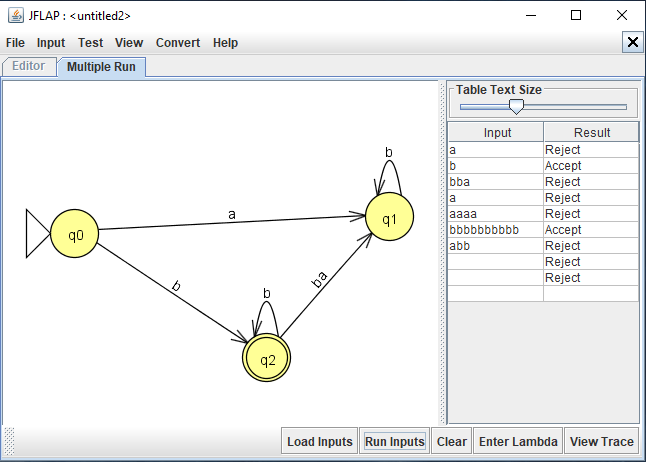
\includegraphics[scale=0.4]{imagenautomata.png}
\end{center}
\newpage

\section{Archivo .json con el automata del ejercicio 1}

\begin{verbatim}
    {
    "name" : "a",
    "representation":{
    "K" : ["q0", "q1", "q2"],
     "A" : ["a","b"],
     "s" : "q0",
     "F" : ["q1"],
     "t" : [["q0", "a", "q1"],
            ["q0", "b", "q2"],
            ["q1", "b", "q1"],
            ["q2", "b", "q2"],
            ["q2", "ba", "q1"]]
}  }
            
      }
\end{verbatim}



\end{document}
